
\chapter{Zusammenfassung und Ausblick}

Im Rahmen dieser Arbeit wurde eine Methodik entwickelt um 
die Deformation, die auf ein Bauteil wirkt, während es eingespannt 
ist optisch zu erkennen. Es wurden additiv gefertigte Bauteile 
betrachtet, da dieser Fertigungsprozess einige Vorteile gegenüber
traditionellen Fertigungsmethoden bietet. 
Vorteil der additiven Fertigung ist zum Beispiel, das hohe Maß der Freiheit und 
Anpassungsmöglichkeit in der Entwicklung eines Bauteils. In der Forschung 
wird oft von der geringen Produktionszeit und dem kleinen Kostenfaktor 
bei wenig Stückzahlen profitiert. Die Deformation eines Bauteils zu 
erkennen ist wichtig, um gewährleisten zu können, dass ein Bauteil für 
den gewünschten Einsatzzweck verwendet werden kann. Zusätzlich können 
durch das entwickelte Verfahren, verschiedene Materialien und Bauteilgeometrien 
auf ihre Verformbarkeit verglichen werden und so ein geeignetes Material 
für das Endprodukt gefunden werden.

\section{Materialunterschiede}

Es zeige sich, dass Metallbauteile deutlich weniger verformt werden als 
Kunststoffe. Zusätzlich wirkt sich die noch im Bauteil vorhanden Stützstruktur 
auf die Deformation des Bauteils auf. 
Interessant ist, dass sich Bauteile mit der gleichen Geometrie, abhängig vom 
Werkstoff unterschiedlich Verformen.
Abbildung \ref{fig:am_fdm_compare} zeigt die Unterschiede in der Deformation 
bei einem additiv gefertigten Metallbauteil zu einem Kunststoffteil mit der gleichen 
Bauteilgeometrie. Es ist zu sehen das sich das Kunststoffteil deutlich mehr verformt.
Zusätzlich ist zu erkennbar, dass die Bauteile sich an unterschiedlichen Stellen verformen.
Das Metallteil wird symmetrisch verformt, die größte Verformung tritt in der Mitte auf.
Das Kunststoffteil verformt sich nicht symmetrisch. Wie in Kapitel \ref{defoinfo} 
bedeutet eine negative Deformation, dass sich das Bauteil nach außen verformt hat.

\begin{figure}[H]
    \centering
    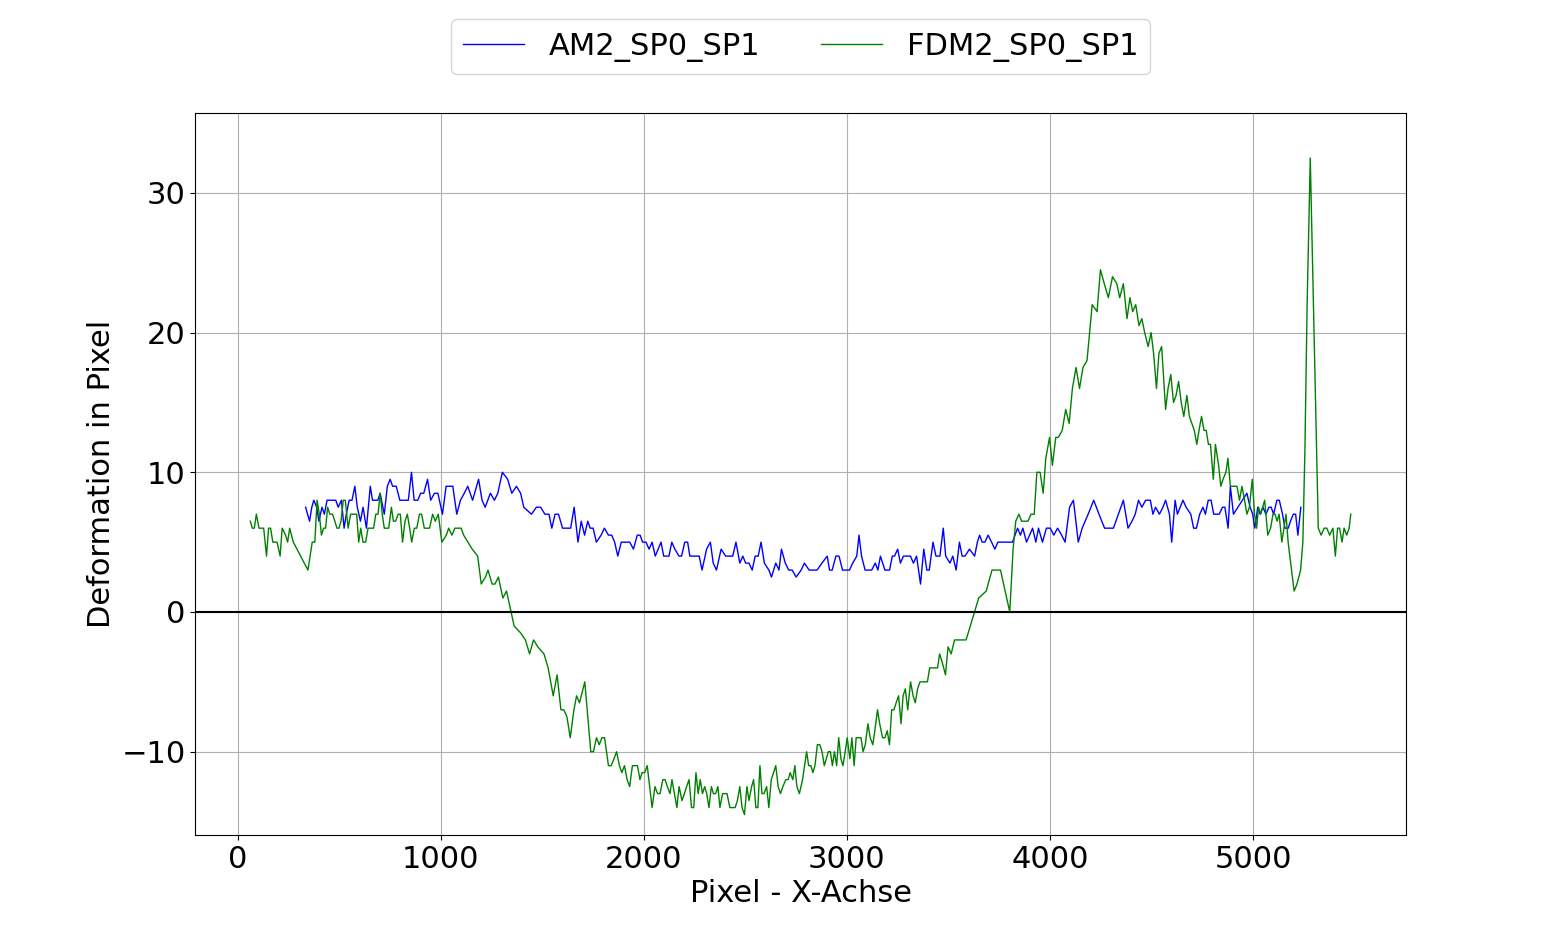
\includegraphics[width=0.9\textwidth]{images/am_fdm.png}
    \caption{Unterschied in der Deformation eines Metallbauteil zu einem
    Kunststoffteil}
    \label{fig:am_fdm_compare}
\end{figure}


\section{Verbesserungspotenzial des Verfahrens}

Das hier entwickelte Verfahren funktioniert grundsätzlich und wurde mithilfe 
eines Demonstratorbauteils umfangreich getestet. Es hat sich gezeigt, dass 
das Stitching sehr große Auswirkungen auf die Deformationerkennung hat. 
Wenn beim Stitching auch nur um ein einzelnes Pixel versetzt transformiert wird,
schlägt sich dieser Fehler direkt in der absolut gemessenen 
Deformation zwischen zwei Spannungsstufen wieder.
Wenn ausreichend Konturen erkannt werden kann die Transformation erfolgreich
berechnet werden, das hat die Anwendung gezeigt. Es kann in dem Stitching-Schritt
aber auch zu Fehler kommen, dieses Fehler auftreten zu beseitigen hat eine hohe Priorität 
bei einer Verbesserung der Methodik. 
Der Fehler kann vermutlich durch eine Verbesserung in der Pointcloud zu Bild 
Konvertierung behoben werden. Diese Verbesserung würde die Ergebnisse 
des Verfahrenes vereinheitlichen. 

\section{Ausblick}

Eine weitere Verbesserung des Verfahrens, könnte sein nicht die Reduktion der 
Scandaten auf zweidimensionale Daten durchzuführen. 
Hierdurch könnte mithilfe von drei Koordinaten das Stitching durchgeführt werden, 
was die Ergebnisse vermutlich auch einheitlich macht. Zusätzlich können 
dann auch Bauteile analysiert werden, die keine flache Oberfläche bieten.
Außerdem kann dann auch die Deformation in Richtung der dritten Achse bestimmt werden. 
Ein weiterer Forschungsansatz ist, dass Verhalten der inneren Struktur eines Bauteils 
während des Einspannvorgangs zu vergleichen. Durch diese Informationen können 
verschiedene innere Strukturen auf ihre Verformbarkeit verglichen und optimiert werden. 

%\begin{itemize}
%    \item Auf die Unterschiede der Materialien eingehen. Auch auf die Ähnlichkeiten 
%    wo die Deformation auftreten.
%    \item Was das für die Bauteile bedeutet.
%    \item Verbesserung: Stitching verbessern, um einheitlichere Ergebnisse zu erhalten.
%    \item Forschungsansätze: Veränderung in der inneren Struktur der Bauteile 
%    vergleichen.
%\end{itemize}
